\section*{3. Galaxy classification}

a) Besides their different morphology, describe the main differences between elliptical and spiral 
galaxies in terms of their kinematics and stellar populations.\\
\\
Spiral galaxies have a defined rotation pattern, while the stars in an elliptical galaxy have a random or
chaotic motion. Elliptical galaxies tend to contain older stars, while spiral galaxies can also contain
younger stars besides old stars. Also elliptical galaxies are gas poor throughout while spiral galaxies
are only gas poor in their halo.\\
\\
b) Based on observations, Edwin Hubble derived a classification scheme for Galaxies, which is known as the
Hubble sequence. The different classes are depicted in the image below.\\
\\
\noindent\makebox[\textwidth]{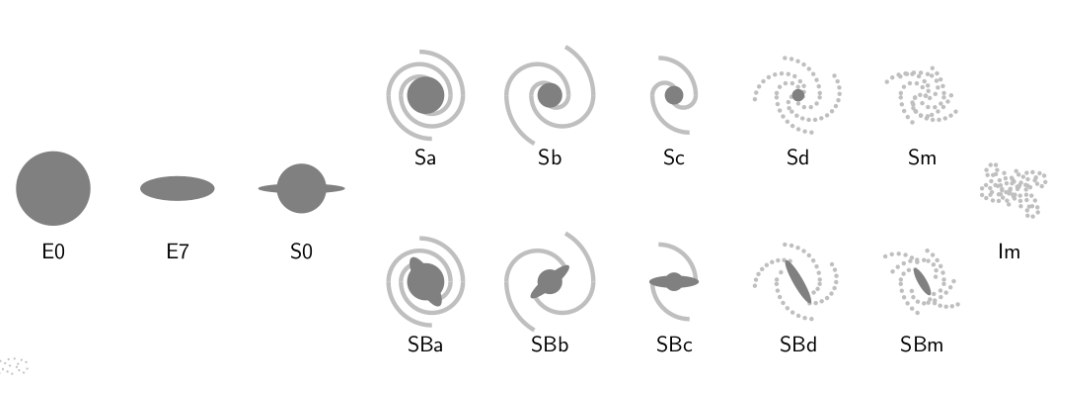
\includegraphics[scale=0.35]{sequence.png}}\\
I.) Use the Hubble scheme, to classify the following real galaxies shown below.\\
\\
\noindent\makebox[\textwidth]{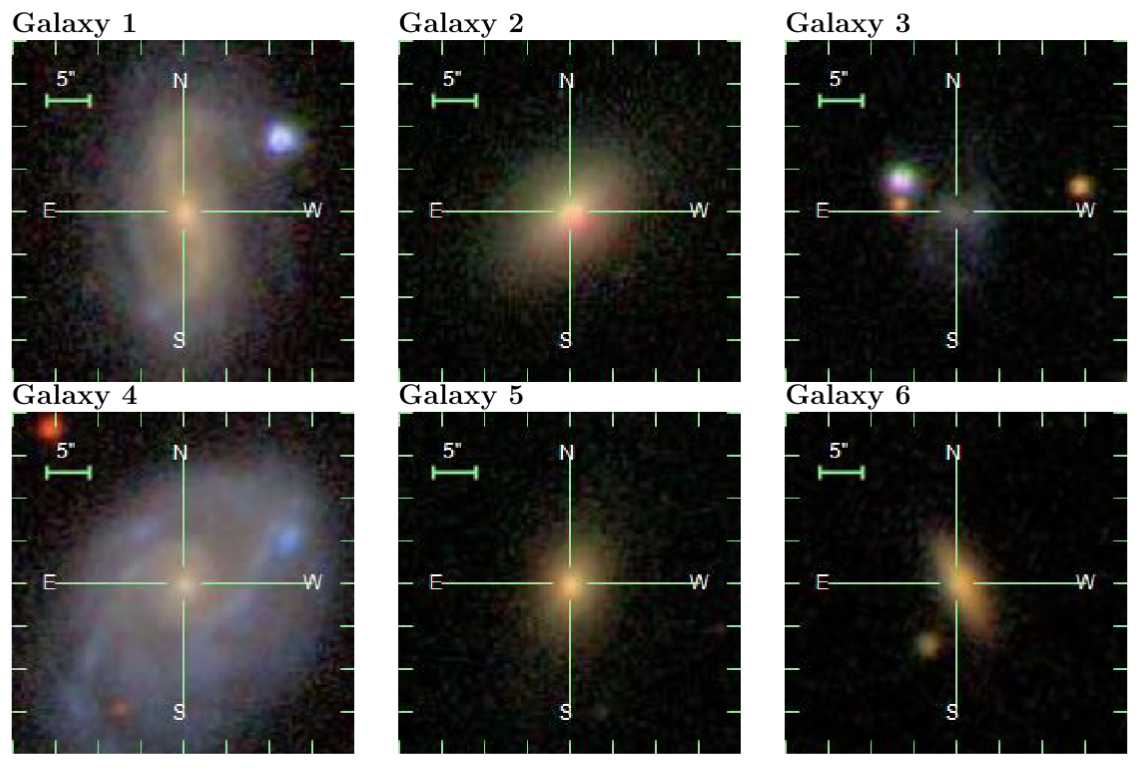
\includegraphics[scale=0.35]{galaxies.png}}\\
\\
\textbf{Galaxy 1:} For this galaxy we can see two well defined tails. We can also see a well defined 
circular center, but the tails only seem to bend after they leave an elliptical extension, which is why
I would classify this galaxy as SBc.\\
\textbf{Galaxy 2:} Again we have a circular center extended by a little less bright ellipses. We can see
that the clusters further away from the center do not form any spiral, which is why I would classify this
galaxy as E7.\\
\textbf{Galaxy 3:} We can only see very blurred non bright cluster, which seem to follow lightly a spiral
pattern. This is why I would classify it as Sm but it could be argued to fit more as a Im.\\
\textbf{Galaxy 4:} Just as the Galaxy 1 we can see two tails emerging from an elliptical extension of the
circular center. This time the pattern is seen more clearly, which is why this is a SBc as well.\\
\textbf{Galaxy 5:} Here we can not see any spiral. The bright center is round and the next outer ring of
that center seems to be very circular as well. The shape of descirbed outer ring can be argued to be
slightly elliptical. But I would classify this as E0 over E7.\\
\textbf{Galaxy 6:} Just as the previous galaxy we can see a similar pattern. This time the outer ring
definetely being elliptical, which is why this is a E7.\\
\\
II.) Describe two shortcomings of the Hubble scheme.\\
\\
The Hubble scheme relies heavily on optical observation, which is why the quality of the image highly
determines the quality of the classification. The provided images had a very poor quality for example and
it was hard to distinguish clusters from one another, which ultimately influenced the ability to find 
patterns like spirals or ellipses. In the same manner it is dependent on the subjectivity of the 
astronomer. It really comes to show when a less bright shape shadows a very well defined shape and it is 
to say if the shape in the background should also be evaluated when trying to match the patterns of the
sequence.
